%\documentstyle[epsf,twocolumn]{jarticle}       %LaTeX2.09仕様
%\documentclass[twocolumn]{jarticle}     %pLaTeX2e仕様
\documentclass[twocolumn]{jarticle}     %pLaTeX2e仕様

%一枚組だったら[twocolumn]関係のとこ消す

\setlength{\topmargin}{-45pt}
%\setlength{\oddsidemargin}{0cm} 
\setlength{\oddsidemargin}{-7.5mm}
%\setlength{\evensidemargin}{0cm} 
\setlength{\textheight}{24.1cm}
%setlength{\textheight}{25cm} 
\setlength{\textwidth}{18.0cm}
%\setlength{\textwidth}{172mm} 
\setlength{\columnsep}{11mm}

\kanjiskip=.07zw plus.5pt minus.5pt

\usepackage{graphicx}
\usepackage[dvipdfmx]{color}
\usepackage{subcaption}
\usepackage{enumerate}
\usepackage{comment}
\usepackage{url}
\usepackage{multirow}
\usepackage{diagbox}
\usepackage{amsmath,amssymb}
\usepackage{mathtools}
\usepackage{wrapfig}
\usepackage{graphicx}
\usepackage{float}
\usepackage{algorithmic}

\usepackage{algorithm}
\usepackage{lipsum}

\begin{document}
\twocolumn[
  \noindent
  \hspace{1em}

  2022 年 12 月 21 日後期研究報告会資料
  \hfill
  \ \  B3 西村昭賢 

  \vspace{2mm}
  \hrule
  \begin{center}
  {\Large \bf カードゲーム型対戦環境への強化学習の適用}
  \end{center}
  \hrule
  \vspace{3mm}
]

\section{はじめに}
近年, 人工知能に関する研究分野は目覚ましい発展を遂げており世の中の様々な分野に応用されている. その中でも人間の脳の働きに近いとされる強化学習と深層学習を組み合わせた深層強化学習は自動運転, ロボット, 推薦システムといった実生活の問題解決に寄与している.\par
深層強化学習はゲームにも盛んに応用されている.
特に将棋や囲碁といった, プレイヤーが意思決定をする段階でそれ以前の意思決定の過程が全て把握可能な完全情報ゲームへの応用が有名である. 
最近では麻雀やポーカーのような, プレイヤーに与えられる情報が部分的である不完全情報ゲームへの応用も注目されている.
\par
そこで, 本研究では不完全情報ゲームであるトレーディングカードゲームを参考にカードゲーム型対戦環境を構築し, 構築環境への強化学習の適用と構築環境のゲームバランスの調整を目標とする. 本稿では対戦環境の構築,強化学習の適用について述べる.

\section{要素技術}

\subsection{OpenAI Gym}
OpenAI Gym は非営利企業 OpenAI が提供する強化学習のシミュレーション用プラットフォームであり, 強化学習の環境として多くのゲームが登録されている\cite{OpenAIGym}. 環境におけるエージェントの行動空間や状態空間, 報酬などを提供されているインターフェースに沿って定義,実装することで自作の環境を登録し利用することができる. シミュレーション環境と強化学習アルゴリズム間のインターフェースが確立されており様々な強化学習用ライブラリに対応しているため比較的容易に強化学習を試すことができる.

\subsection{Q学習}
強化学習では,エージェントが行動することで環境から報酬を得る. 強化学習における行動はその直後に獲得する報酬の大きさではなく, 未来に渡っての報酬の総和を見積もった値である「価値」の最大化に繋がるかという観点で評価される.
価値の最大化を目指す場合にはある状態 $s$ において行動 $a$ をとったときの価値が分かれば良い.この価値のことを Q 値, あるいは行動価値関数と呼ぶ.
 Q 学習ではエージェントの 1 ステップごとに (\ref{updateQ}) 式に示す更新式で Q 値を更新する.
\begin{equation}
  \small
  \label{updateQ}
  Q(s_t,a_t) \leftarrow  Q(s_t,a_t) + \alpha(r_{t+1} + \gamma \mathrm{max}_{a_{t+1}}Q(s_{t+1},a_{t+1}) - Q(s_t,a_t))
\end{equation}
なお $t$ は時間, $r$ は報酬, $\alpha$ は学習率, $\gamma$ は割引率を表す.

\subsection{Deep Q Network}
Q 学習では実装の際に Q 値のテーブルを作成する.しかし状態空間や行動空間が高次元である, あるいは状態や行動が離散値ではなく連続値で表現される場合 Q テーブルのメモリ量は爆発してしまう.この問題を解決した技術が Deep Q Network (DQN) である.
 DQN ではニューラルネットワークを用いて, ある状態における行動ごとの Q 値を推定する.エージェントが経験した過去の体験を Replay Memory に一定期間保存しておき, 過去の経験をランダムにサンプリングして学習する Experience Replay や,行動を決定する Q 値のネットワークと Q 値の学習を行うネットワークを分けることで Q 値の過大評価を防ぐ Fixed Target Network といった工夫により安定した学習を可能としている\cite{DQN}.

\subsection{モンテカルロ探索}
モンテカルロ探索 (Monte Carlo Search ; MCS) は Q 学習と同様に Q 値を推定する学習アルゴリズムであるが, Q 学習のように 1 ステップごとに Q 値を更新するのではなく, 1 エピソードをランダムに行動し, 終了状態に到達してから辿ったステップ $t$ = 1 $\sim$ T $-$ 1 について Q 値を更新する. Q 値の更新は学習率 $\alpha$ , 割引率 $\gamma$ ,エピソードから得られた割引現在価値 $G_t$ を用いて (\ref{montecarlo}) 式に従う.
\begin{eqnarray}
  \label{montecarlo}
  &Q(s_t,a_t) \leftarrow (1 - \alpha)Q(s_t,a_t) + \alpha * G_{t} \\
  \mathrm{where}  &G_t = r_{t+1} + \gamma r_{t+2} + ... + \gamma^{\mathrm{T}-t-1} r_{t+k+1} \nonumber
\end{eqnarray}


\section{カードゲーム型対戦環境の構築}
\subsection{トレーディングカードゲーム}
今回の実験で構築したカードゲーム型対戦環境は, HearthStone \footnote[1]{https://hearthstone.blizzard.com/ja-jp}や Shadowverse \footnote[2]{https://shadowverse.jp/} といったトレーディングカードゲーム (Trading Card Game ; TCG) を参考にした. TCG は 2 人のプレイヤーによりプレイされるゲームである. 囲碁や将棋のようにプレイヤーは先攻と後攻に分かれ, ターン制で進んでいく. 
ゲームタイトルごとに細かいルールは異なるが, 相手プレイヤーのカードの 1 部分はプレイヤーから観測できない不完全情報ゲームである.

\subsection{構築環境}
実装したカードゲームのルール, 用語を説明する.
ゲームは 2 人のプレイヤーからなり, プレイヤーは複数のカードからなるデッキを持つ.
プレイヤーは手札, 盤面と呼ばれるカードを保有する領域を持ち, ドローと呼ばれる操作でカードをデッキから手札に加える. また,プレイと呼ばれる操作でカードを手札から盤面に出す.また, デッキからカードが無くなった状態をデッキ切れと呼ぶ.
\par
カードはそれぞれ攻撃力と HP の 2 つの数値を持つ. カードは盤面にある時に対戦相手の盤面にあるカードに攻撃することができる.ただし, カードの攻撃が可能となるのはカードがプレイされたターンの次のターンからになる. カードが攻撃を行う際には, 相手盤面に存在する攻撃対象のカードの HP へ自身の攻撃力分ダメージを与える. HP が 0 になればそのカードは破壊される. またカードが攻撃する際には, 攻撃対象のカードの攻撃力分自身もダメージを受ける.

\subsection{ゲームフロー}
\begin{enumerate}
  \setlength{\itemsep}{0cm} % 項目間
  \item ゲーム開始時に各プレイヤーは自身のデッキをシャッフルする.
  \item デッキからカードを 3 枚ドローする.
  \item 先攻プレイヤーは 1 ターン目の行動をする.
  \item 後攻プレイヤーはカードを 1 枚ドローして行動する.
  \item 2 ターン目以降は先攻プレイヤーもカードを 1 枚ドローしてから行動する.
  \item 4 , 5 を繰り返す.
  \item どちらかのプレイヤーがデッキ切れになっている状態で, カードをドローしようとしたらゲーム終了となる.
\end{enumerate}
勝利条件は 4.3 節で述べる.
本構築環境では, 一般的な TCG と同様に先攻プレイヤーがカードの行動が早いため有利となる.そのため, 1 ターン目のドローといったメリットを後攻に加えている. 

\section{実験}
構築環境へ強化学習が適用できるか検証した.
強化学習手法として DQN , MCS の 2 つを用いた. 2 つの手法について構築環境において後攻のプレイヤーとして同程度学習し, 学習後に学習済みのモデルを用いて 10000 回ゲームを行い勝率を計算した.また, 学習が進んでいるかどうか判断するため学習時の獲得報酬の推移を記録した.

\subsection{対戦相手の行動ルーチン}

学習,勝率計算の際は学習するプレイヤーの対戦相手となるプレイヤーを用意する必要がある.
Algorithm \ref{alg1} に今回の実験における対戦相手の行動ルーチンを示す.
\begin{figure}[H]
  \begin{algorithm}[H]
      \caption{
        対戦相手の行動ルーチン
        }
      \label{alg1}
      \begin{algorithmic}[1] 
      \STATE 盤面にカードを 1 枚プレイ
      \FOR{盤面のカード (プレイ順が古い方から)}
      \IF{敵の盤面にカードがある}
      \STATE ランダムに攻撃対象を選んで攻撃
      \ELSE
      \STATE 何もしない
      \ENDIF
      \ENDFOR
      \STATE ターンを終了
      \end{algorithmic}
  \end{algorithm}
  \end{figure}


\subsection{デッキ}
学習側,対戦相手ともに同じデッキを持つ.
デッキの内容は表 \ref{table:deck} に示す.
\begin{table}[H]
  \centering
  \caption{デッキの内容}
  \label{table:deck}
  \vspace{-0.3cm}
  \scalebox{0.9}[0.9]{
    \begin{tabular}{|c|c|c|}
      \hline
      攻撃力 &  HP  & 枚数 \\ \hline \hline
      3 & 3 & 5  \\ \hline
      2 & 4 & 5  \\ \hline
      2 & 3 & 5  \\ \hline
      \end{tabular}
  }
  \end{table}

\subsection{勝利条件}
ゲーム終了時に.\par
(学習側盤面の枚数) $>$ (対戦相手盤面枚数)ならば,\par
学習側の勝利.\par 
(学習側盤面の枚数) $\leq$ (対戦相手盤面枚数)ならば,\par
対戦相手の勝利とした.\par 

\subsection{報酬の定義}
報酬は以下のように設定した.\par
1 ステップ終了後 
\begin{equation*}
 \mathrm{reward} = 0.0  
\end{equation*}
\par
1 エピソード終了後 
\begin{equation*}
  \mathrm{reward} = 
  \left\{
    \begin{aligned}
        1.0 \quad & (学習プレイヤーの勝利) \\
        -1.0 \quad & (敵プレイヤーの勝利) \\
    \end{aligned}
    \right.
\end{equation*}

\subsection{状態空間と行動空間の定義}
強化学習では, エージェントの取りうる行動と観測できる状態の空間を定義する必要がある. 
TCG ではドローやプレイ, カードの攻撃による破壊といった行動で盤面や手札の枚数が変化する場合があり, 各ステップ時点で取りうる行動の次元を計算するとステップごとに空間の次元が変わり学習が行えない.\par
そのため本研究では予め手札と盤面の枚数の上限をそれぞれ 9 枚, 5 枚と定め , 手札と盤面に存在するカードに自盤面 1 というように番号をつけ, カードが存在しない場合は状態を 0 とすることで状態空間と行動空間の定義に成功した. 表 \ref{table:state} , \ref{table:action} に状態空間, 行動空間の定義を示す.
なお,ドローやプレイといった操作でカードを追加し枚数の上限を超える場合には追加しようとしたカードを破壊する. \par
また,学習側は表 \ref{table:action} に基づいて, 保有している手札と盤面のカード全てについて盤面に出すか出さないか, 攻撃するかしないかを行動し終えた段階でターンエンドとする.


\begin{table}[H]
  \centering
  \caption{定義した状態空間}
  \label{table:state}
  \vspace{-0.3cm}
  \scalebox{0.85}[0.85]{
    \begin{tabular}{|c|c|c|c|}
      \hline
      状態説明                        & 次元数        & 最小値        & 最大値         \\ \hline \hline
      \begin{tabular}{c}
        手札 1 $\sim$ 9 の\\HP と攻撃力
        \end{tabular}      & 18         & 0          & 20          \\
      \hline
      \begin{tabular}{c}
        自盤面 1 $\sim$ 5 の\\HP と攻撃力
      \end{tabular}     & 10         & 0          & 20 \\
      \hline
      \begin{tabular}{c}
        敵盤面 1 $\sim$ 5 の\\HP と攻撃力
      \end{tabular}     & 10         & 0          & 20 \\
      \hline
      \begin{tabular}{c}
        自盤面 1 $\sim$ 5 が\\攻撃可能かどうか
      \end{tabular} & 5          & 0          & 1  \\
      \hline
      \begin{tabular}{c}
        お互いのデッキの\\残り枚数
      \end{tabular}     & 2 & 0 & 15 \\
       \hline
      \end{tabular}
  }
  \end{table}

  \begin{table}[H]
    \centering
    \caption{定義した行動空間}
    \vspace{-0.3cm}
    \label{table:action}
    \scalebox{0.9}[0.9]{
      \begin{tabular}{|c|c|}
        \hline
        行動説明                          & 次元数        \\ \hline \hline
        手札 1 $\sim$ 9 を自盤面に出す             & 9          \\ \hline
        手札 1 $\sim$ 9 を自盤面に出さない & 9 \\ \hline
        自盤面 1 が敵盤面 1 $\sim$ 5 に攻撃or何もしない    & 6          \\ \hline
        自盤面 2 が敵盤面 1 $\sim$ 5 に攻撃or何もしない    & 6          \\ \hline
        自盤面 3 が敵盤面 1 $\sim$ 5 に攻撃or何もしない    & 6          \\ \hline
        自盤面 4 が敵盤面 1 $\sim$ 5 に攻撃or何もしない    & 6          \\ \hline
        自盤面 5 が敵盤面 1 $\sim$ 5 に攻撃or何もしない    & 6          \\ \hline
        \end{tabular}
    }
    \end{table}
  
  \subsection{DQN, MCS のパラメータ}
  表 \ref{table:dqnparam} , \ref{table:mcsparam} に実験で用いた 2 種の強化学習アルゴリズムのパラメータを示す.
  \begin{table}[H]
    \centering
    \caption{DQNのパラメータ}
    \vspace{-0.3cm}
    \label{table:dqnparam}
    \scalebox{0.95}[0.95]{
      \begin{tabular}{|c|c|}
        \hline
        パラメータ名 & 値 \\ \hline \hline
        割引率 $\gamma$ & 0.99 \\ \hline     
        全結合層の活性化関数             & ReLU     \\ \hline
        全結合層の次元                & 64       \\ \hline
        最適化アルゴリズム              & Adam     \\ \hline
        方策                 & ε-greedy \\ \hline
        ε & 0.1 \\ \hline  
        Target Network 更新重み              & 0.5     \\ \hline
        Exprience Memory 開始ステップ数 & 10000 \\ \hline
        学習ステップ数 & 5000000 \\ \hline
        \end{tabular}
    }
    \end{table}
  
    \begin{table}[H]
      \centering
      \caption{MCSのパラメータ}
      \vspace{-0.3cm}
      \label{table:mcsparam}
      \scalebox{0.95}[0.95]{
        \begin{tabular}{|c|c|}
          \hline
          パラメータ名 & 値 \\ \hline \hline
          学習率 $\alpha$ & 0.5 \\ \hline
          割引率 $\gamma$ & 0.99 \\ \hline     
          学習エピソード数 & 85000 \\ \hline
    
          \end{tabular}
      }
      \end{table}


\section{結果}
表 \ref{table:result} に実験結果を示す. なお,ベースラインとして対戦相手と同じ戦略のプレイヤーを後攻に配置し 10000 回対戦し勝率を計算した.
\begin{table}[H]
  \centering
  \caption{実験結果}
  \vspace{-0.3cm}
  \label{table:result}
  \scalebox{0.9}[0.9]{
    \begin{tabular}{|c|c|}
      \hline
      手法 & 勝率 \\ \hline \hline
      DQN & 0.9069 \\ \hline
      MCS & 0.7257 \\ \hline     
      対戦相手と同じ戦略 & 0.1294 \\ \hline

      \end{tabular}
  }
  \end{table}

  図 \ref{fig:MCSresult} , \ref{fig:DQNresult} に学習過程のグラフを示す.図中の緑点は 学習時の100 エピソードにおける平均獲得報酬を表し,薄緑の領域は分散を示している.
  また縦軸は reward ,横軸はエピソード数を示している. 

  \begin{figure}[H]
    \centering
    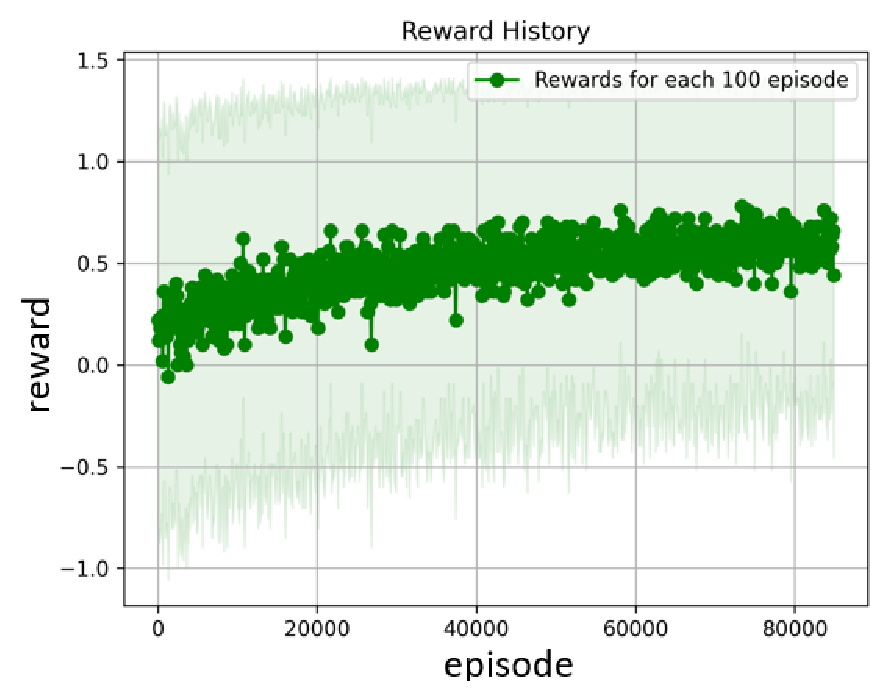
\includegraphics[width=85mm]{assets/MCS_update.eps.eps}
    \caption{MCS における平均獲得報酬の推移}
    \label{fig:MCSresult}
  \end{figure}

  \begin{figure}[H]
    \centering
    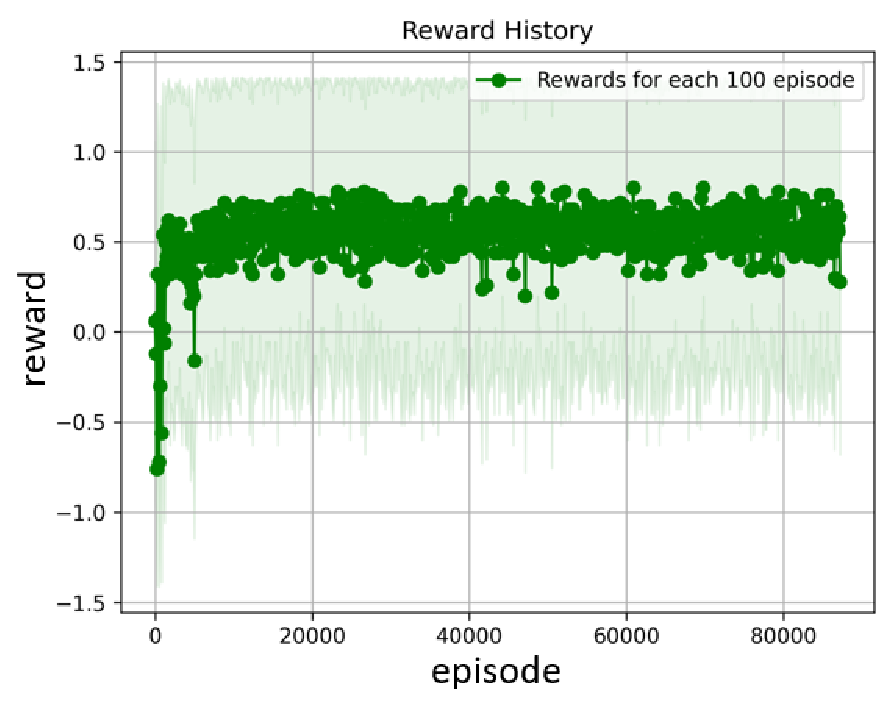
\includegraphics[width=83.5mm]{assets/DQN_update.eps}
    \caption{DQN における平均獲得報酬の推移}
    \label{fig:DQNresult}
  \end{figure}
DQN , MCS 共にベースラインに比べ遥かに高い勝率を記録している.特に, DQN は 約 9 割もの勝率を記録している.
図 \ref{fig:MCSresult} から, 学習が進んでいくにつれ平均獲得報酬が増加しており構築環境において強化学習が適用できていることが分かる.
また, 図 \ref{fig:DQNresult} に示すMCS より高い勝率を記録した DQN の推移からは, MCSに比べて短いエピソード数で学習が安定していることが分かる.
  

\section{まとめと今後の課題}
今回の実験では簡易的なルールにおけるカードゲーム型対戦環境の構築を行った.
また, 構築環境に強化学習を適用し, 高い勝率を記録することができた.
\par
今後の課題として,研究の最終目的であるカードゲーム型対戦環境のゲームバランス調整に取り組むことが挙げられる.\par
また, 一般的な TCG ではプレイヤー自身に HP を定義しカードがプレイヤーに攻撃できるようにする, カードにコストというパラメータを設けて盤面にプレイする際に制約を設けるといった仕様を加えることでよりゲームの戦略性を深めている. \par
今回作成した環境はゲームの終了条件と勝利条件が直接関係していない, 1ターンに出そうと思えば何枚もカードをプレイできるといったようにゲームデザインが詰めきれていない. カードのコストやプレイヤーの HP といった仕様を構築環境に取り入れ, より戦略性の高いカードゲーム型対戦環境を作成することも今後の課題である.




%index.bibはtexファイルと同階層に置く
%ちゃんと\citeしないと表示されない(1敗)
\bibliography{index.bib}
\bibliographystyle{junsrt}

\end{document}